\documentclass[paper=a4, 
                DIV=12]{scrartcl}
\usepackage[ngerman]{babel} % Deutsche Sprache
\usepackage[utf8]{inputenc}
\usepackage{graphicx} % Required for inserting images
\usepackage{matlab-prettifier}
\usepackage{amsmath}
\usepackage{amsfonts}
\usepackage{float}
\usepackage{scrlayer-scrpage}

\newcommand{\thesisauthor}{Timo Johannsen \\ Benjamin Peiter \\ Omer Butt}
\newcommand{\thesiscourse}{Einführung in MATLAB und Simulink}
\newcommand{\thesisstudy}{Informatik - Künstliche Intelligenz - TIK24}

\newcommand{\thesistype}{Programmentwurf}
\newcommand{\thesistitle}{Programmentwurf zur Vorlesung „Einführung in MATLAB und Simulink“}
\newcommand{\thesisdate}{27.04.2025}

\begin{document}

\begingroup
    \begin{flushright} % Aligns content to the right
        
\includegraphics[height=1.5cm]{figures/dhbw.png}
    \end{flushright} 
    \centering
    \vspace*{0.5cm}
    \Large
    \textbf{\thesistitle} \\
    \vspace*{3cm}
    \normalsize
    \thesistype \\
    \vspace*{2.5cm}
    des Studienganges \thesisstudy \\
    an der Dualen Hochschule Baden-Württemberg Ravensburg Standort Friedrichshafen\\
    \vspace*{2.5cm}
    von \\
    \thesisauthor \\
    \vfill
    \thesisdate\\
    \vspace*{1cm}
    \textbf{Kurs:} \thesiscourse\\
    \normalsize

\endgroup

\newpage
\tableofcontents
\newpage

\section{Aufgabe (a): Visualisierung der Systemdynamik durch Phasenportraits}
Zu der \textit{Tschirikow Standardabbildung}, welche definiert ist durch:
\begin{gather*}
    F: [0,2\pi] \times [0,2\pi] \to [0,2\pi] \times [0,2\pi] \\
    F(I, \theta) = 
    \begin{pmatrix}
        I + K \cdot \sin(\theta) \bmod 2\pi \\
        I + \theta + K \cdot \sin(\theta) \bmod 2\pi
    \end{pmatrix}
\end{gather*}
gehört ein dynamisches System, welche gegeben ist durch die Rekursionsgleichungen
\begin{gather*}
    I_{n+1} = (I_n + K \cdot \sin(\theta_n)) \bmod 2\pi \\
    \theta_{n+1} = (\theta_n + I_n) \bmod 2\pi
\end{gather*}

\noindent Zuerst werden 3 verschiedene K-Werte mit $K_{1} = ]0,0.6]$, $K_{2} = [0.9,1.1]$ und \hbox{$K_{3} = [1.4,2.0]$} gewählt und die Länge und Anzahl der Trajektorien definiert. 
\begin{lstlisting}[frame=single, style=Matlab-editor]
K_values = [rand()*0.6, 0.9 + rand()*0.2, 1.4 + rand()*0.6];
    % Parameter fuer die drei K-Werte
N = 1000; % Laenge der Trajektorien
M = 50; % Anzahl der Trajektorien
\end{lstlisting}
Daraufhin werden für die 3 K-Werte die Phasenportraits erstellt. In einer Schleife werden durch die K-Werte iteriert und für jeden K-Wert die Trajektorien gezeichnet.
\begin{lstlisting}[frame=single, style=Matlab-editor]
figure;
for idx = 1:3
    K = K_values(idx);
    subplot(1,3,idx);
    hold on;
\end{lstlisting}
Jede Trajektorie bekommt eine zufälligen Startpostition $(I_0, \theta_0)$ aus dem Bereich \hbox{$[0,2\pi]$ x $[0,2\pi]$}.
Zusätzlich wird für die Trajektorie zwei Vektoren der Länge 1000 erstellt, in der die Werte für $I$ und $\theta$ gespeichert werden.
\begin{lstlisting}[frame=single, style=Matlab-editor]
    for m = 1:M
        I = rand()*2*pi;
        theta = rand()*2*pi;
        I_traj = zeros(1,N);
        theta_traj = zeros(1,N);
\end{lstlisting}
Die Trajektorie wird dann rekursiv berechnet. Dabei werden die Formeln:
\begin{gather*}
    I_{n+1} = (I_n + K \cdot \sin(\theta_n)) \bmod 2\pi \\
    \theta_{n+1} = (\theta_n + I_n) \bmod 2\pi
\end{gather*}
verwendet, wobei $I$ und $\theta$ in jedem Schritt aktualisiert werden. Die Trajektorie wird dann in den Vektoren gespeichert und zum Schluss wird jeder Punkt gezeichnet.
\newpage
\begin{lstlisting}[frame=single, style=Matlab-editor]
        for n = 1:N
            I = mod(I + K*sin(theta), 2*pi);
            theta = mod(theta + I, 2*pi);
            I_traj(n) = I;
            theta_traj(n) = theta;
        end
        plot(theta_traj, I_traj, '.', 'MarkerSize', 1);
    end
\end{lstlisting}
Diese Werte werden dann in einem Diagramm gezeichnet. Dabei wird die x-Achse mit $\theta$ und die y-Achse mit $I$ beschriftet.
\noindent Dabei charakterisieren die Phasenportraits die Dynamik des Systems, dass für ein wachsendes K das chaotische Verhalten zunimmt. \\
\begin{figure}[H]
    \centering
    \begin{minipage}[t]{0.48\textwidth}
        \centering
        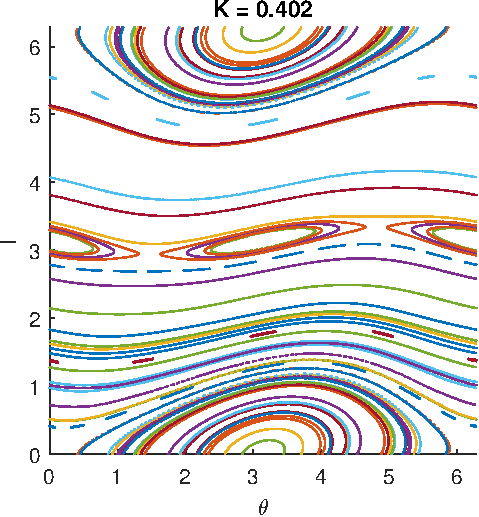
\includegraphics[height=0.28\textheight]{figures/phasenportrait_k1.pdf}
        \caption{Phasenportrait für $K_1$}
    \end{minipage}
    \hfill
    \begin{minipage}[t]{0.48\textwidth}
        \centering
        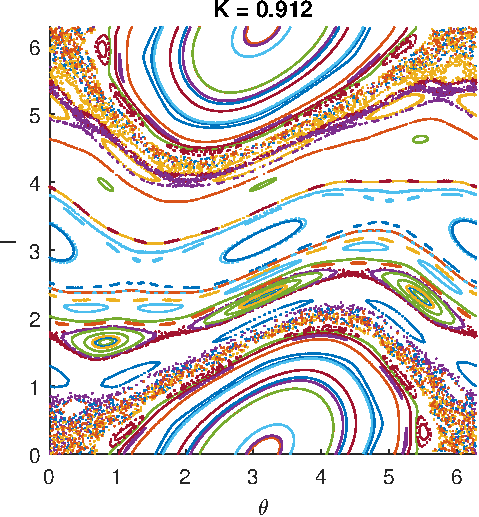
\includegraphics[height=0.28\textheight]{figures/phasenportrait_k2.pdf}
        \caption{Phasenportrait für $K_2$}
    \end{minipage}
    \par\vspace{1cm}
    \begin{minipage}[t]{0.48\textwidth}
        \centering
        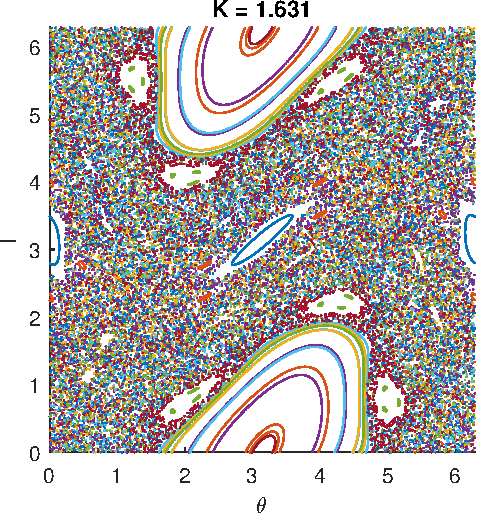
\includegraphics[height=0.28\textheight]{figures/phasenportrait_k3.pdf}
        \caption{Phasenportrait für $K_3$}
    \end{minipage}
\end{figure}

\newpage
\section{Aufgabe (b): Quantifizierung des Chaos durch Ljapunov-Exponenten}
Die Ljapunov-Exponenten zeigen das Ausmaß an chaotischem Verhalten eines Systems quantifiziert an.
Dafür werden im gleichmäßigen Abstand 200 K-Werte zwischen 0 und 4 gewählt. 
\begin{lstlisting}[frame=single, style=Matlab-editor]
K_vals = linspace(0, 4, 200);
N = 1000;
lambda1 = zeros(size(K_vals));
lambda2 = zeros(size(K_vals));
\end{lstlisting}
Für jeden K-Wert wird eine Trajektorie mit einer zufälligen Startposition $(I_0, \theta_0)$ aus dem Bereich \hbox{$[0,2\pi]$ x $[0,2\pi]$} erstellt.
$Q$ ist anfangs eine Einheitsmatrix, die später in der QR-Zerlegung aktualisiert wird. $sumLogR11$ und $sumLogR22$ sind die Summen der Logarithmen der ersten beiden Diagonalelemente der Matrix $R$, die aus der QR-Zerlegung resultiert.
\begin{lstlisting}[frame=single, style=Matlab-editor]
for idx = 1:length(K_vals)
    K = K_vals(idx);
    I = rand()*2*pi;
    theta = rand()*2*pi;
    Q = eye(2);
    
    sumLogR11 = 0;
    sumLogR22 = 0;
\end{lstlisting}
Die Ljapunov-Exponenten werden dann mit der berechneten Trajektorie berechnet. 
Dabei wird die \textit{Systemmatrix} $DF$ erstellt, welche die Ableitung der \textit{Standardabbildung} $F$ ist.
\begin{gather*}
    DF = \begin{pmatrix}
        1 & K \cdot \cos(\theta) \\
        1 & 1 + K \cdot \cos(\theta)
    \end{pmatrix}
\end{gather*}
\begin{lstlisting}[frame=single, style=Matlab-editor]
    for n = 1:N
        % Ableitungsmatrix DF
        DF = [1, K*cos(theta); 1, 1 + K*cos(theta)];
\end{lstlisting}
Um die Ljapunov-Exponenten zu berechnen, wird die QR-Zerlegung der Matrix $A$ durchgeführt, die aus der Ableitungsmatrix $DF$ und der Matrix $Q$  rekursiv resultiert.
Dafür werden diese Rekursionsgleichungen aufgestellt:
\begin{gather*}
    Q_0 =
    \begin{pmatrix}
        1 & 0 \\
        0 & 1
    \end{pmatrix} \\
    A_{n+1} = DF(I_n, \theta_n) \cdot Q_n = 
    \begin{pmatrix}
        1 & K \cdot \cos(\theta) \\
        1 & 1 + K \cdot \cos(\theta)
    \end{pmatrix} \cdot Q_n \\
    A_{n+1} = Q_{n+1} \cdot R_{n+1}
\end{gather*}
Dabei ist $Q_{n+1} \cdot R_{n+1}$ die QR-Zerlegung der Matrix $A_{n+1}$.
\begin{lstlisting}[frame=single, style=Matlab-editor]
        A = DF * Q;
        [Q, R] = qr(A);
\end{lstlisting}
\newpage
Die Ljapunov-Exponenten $\lambda_i, i = 1,2$ sind dann gegeben durch:
\begin{gather*}
    \lambda_i = \lim_{N\to\infty}\frac{1}{N}\sum_{n=0}^{N-1}ln((R_n)_{ii})
\end{gather*}
Dann werden die $I_n$ und $\theta_n$ entsprechend einer Trajektorie aktualisiert.
\begin{lstlisting}[frame=single, style=Matlab-editor]
        sumLogR11 = sumLogR11 + log(abs(R(1,1)));
        sumLogR22 = sumLogR22 + log(abs(R(2,2)));

        I = mod(I + K*sin(theta), 2*pi);
        theta = mod(theta + I, 2*pi);
    end
\end{lstlisting}
Um die Ljapunov-Exponenten zu erhalten, wird die Summe der Logarithmen der Diagonalelemente $sumLogR11$ und $sumLogR22$, durch die Länge der Trajektorie $N$ geteilt. 
\begin{lstlisting}[frame=single, style=Matlab-editor]
    lambda1(idx) = sumLogR11 / N;
    lambda2(idx) = sumLogR22 / N;
end
\end{lstlisting}
Diese Exponenten werden dann für jeden K-Werte in einem Diagramm gezeichnet.
\begin{figure}[H]
    \centering
    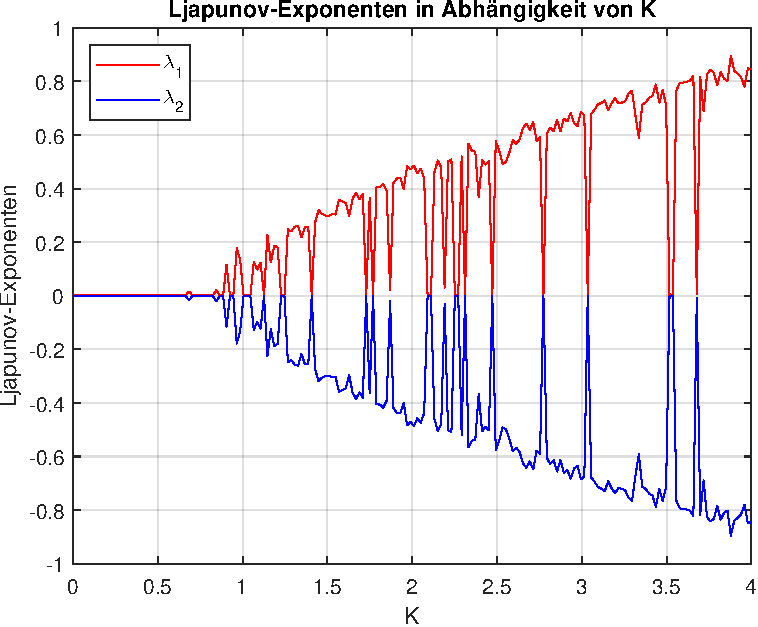
\includegraphics[width=0.8\textwidth]{figures/exponenten.pdf}
    \caption{Ljapunov-Exponenten}
\end{figure}
\newpage
\section{Aufgabe (c): Plausibilisierung der Ergebnisse aus (b)}
\textbf{1. Determinante der Systemmatrix $DF(I, \theta)$:} \\
Die Matrix $DF(I, \theta)$ ist gegeben durch:
\begin{gather*}
    DF(I, \theta) = \begin{pmatrix}
        1 & K \cdot \cos(\theta) \\
        1 & 1 + K \cdot \cos(\theta)
    \end{pmatrix}
\end{gather*}
Die Determinante dieser Matrix ist dann:
\begin{eqnarray*}
    det(DF) &=& (1 \cdot (1 + K \cdot \cos(\theta))) - (K \cdot \cos(\theta) \cdot 1) \\
    &=& 1 + K \cdot \cos(\theta) - K \cdot \cos(\theta) \\
    &=& 1
\end{eqnarray*}
Die Determinante der Systemmatrix ist unabhängig von $K$ und $\theta$ und beträgt immer 1. \\

\noindent\textbf{2. Determinante von $Q_n$:} \\
Da die Matrix $Q_n$ für alle $n \in \mathbb{N}$ eine orthogonale Matrix ist, gilt:
$$ det(Q_n) = \pm 1 $$

\noindent\textbf{3. Folgerung für $det(A_n)$}: \\
Da $A_n = DF \cdot Q_n$ gilt, ist die Determinante von $A_n$ gegeben durch:
\begin{eqnarray*}
    det(A_n) &=& det(DF) \cdot det(Q_n) \\
    &=& 1 \cdot (\pm 1) \\
    &=& \pm 1  
\end{eqnarray*}

\noindent\textbf{4. Folgerung für $det(R_n)$:} \\
Da $A_n = Q_n \cdot R_n$ gilt, ist die Determinante von $A_n$ gegeben durch:
\begin{eqnarray*}
    det(A_n) &=& det(Q_n) \cdot det(R_n) \\
    \pm 1 &=& \pm 1 \cdot det(R_n) \\
    det(R_n) &=& \pm 1
\end{eqnarray*}

\noindent\textbf{5. Diagonalelement von $R_n$}: \\
Da $R_n$ eine obere Dreiecksmatrix mit positiven Diagonalelement ist gilt:
$$ det(R_n) = (R_n)_{11} \cdot (R_n)_{22} = 1$$

\noindent\textbf{6. Wert von $ln((R_n)_{11}) + ln((R_n)_{22})$:} \\
Da $ln(a \cdot b) = ln(a) + ln(b)$ gilt, ist:
\begin{eqnarray*}
    ln((R_n)_{11}) + ln((R_n)_{22}) &=& ln((R_n)_{11} \cdot (R_n)_{22}) \\
    &=& ln(1) \\
    &=& 0
\end{eqnarray*}

\newpage
\noindent\textbf{7. Folgerung für die Ljapunov Exponenten $\lambda_1$ und $\lambda_2$:} \\
Die Exponenten sind definiert durch: 
$$ \lambda_i = \lim_{N\to\infty}\frac{1}{N}\sum_{n=0}^{N-1}ln((R_n)_{ii}) $$
Die Summe von $\lambda_1$ und $\lambda_2$ ist somit gegeben durch:
\begin{eqnarray*}
    \lambda_1 + \lambda_2 &=& \lim_{N\to\infty}\frac{1}{N}\sum_{n=0}^{N-1}[ln((R_n)_{11}) + ln((R_n)_{22})] \\
    &=& \lim_{N\to\infty}\frac{1}{N}\cdot 0 \\
    &=& 0
\end{eqnarray*}
Das heißt, dass die Exponenten symmetrisch sind und heben sich gegenseitig auf:
$$ \lambda_1 = -\lambda_2 $$
Dies ist auch in dem Diagramm zu sehen:
\begin{figure}[H]
    \centering
    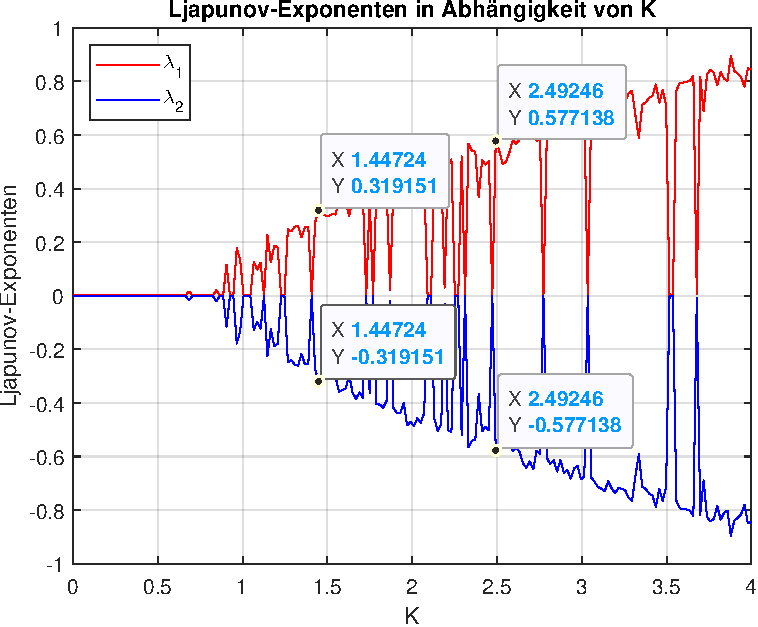
\includegraphics[width=0.8\textwidth]{figures/exponenten_data.pdf}
    \caption{Ljapunov-Exponenten}
\end{figure}
\end{document}
